\documentclass[12pt]{exam}

\usepackage[utf8]{inputenc}  % For UTF8 source encoding.
\usepackage{amsmath}  % For displaying math equations.
\usepackage{amsfonts} % For mathematical fonts (like \mathbb{E}!).
\usepackage{upgreek}  % For upright Greek letters, such as \upvarphi.
\usepackage{wasysym}  % For additional glyphs (like \smiley!).
\usepackage{mathrsfs} % For script text (hash families and universes).
\usepackage{enumitem}
\usepackage{graphicx}
% For document margins.
\usepackage[left=.8in, right=.8in, top=1in, bottom=1in]{geometry}
\usepackage{lastpage} % For a reference to the number of pages.
\usepackage[table,xcdraw]{xcolor}
\usepackage{pdfpages}
\usepackage{verbatim}

% TODO: Enter your name here :)
\newcommand*{\authorname}{Luis A. Perez}

\newcommand*{\duedate}{Wednesday, July 17th}
\newcommand*{\duetime}{11:59 pm}

% Fancy headers and footers
\headrule
\firstpageheader{EE 263\\Summer 2019}{Homework 3 \\ }{Due: \duedate\\at \duetime}
\runningheader{EE 263}{Homework 3}{\authorname}
\footer{}{\footnotesize{Page \thepage\ of \pageref{LastPage}}}{}

% Exam questions.
\newcommand{\Q}[1]{\question{\large{\textbf{#1}}}}
\qformat{}  % Remove formatting from exam questions.

% Useful macro commands.
\newcommand*{\bigtheta}[1]{\Theta\left( #1 \right)}
\newcommand*{\bigo}[1]{O \left( #1 \right)}
\newcommand*{\bigomega}[1]{\Omega \left( #1 \right)}
\newcommand*{\prob}[1]{\text{Pr} \left[ #1 \right]}
\newcommand*{\ex}[1]{\text{E} \left[ #1 \right]}
\newcommand*{\var}[1]{\text{Var} \left[ #1 \right]}

\newcommand*{\norm}[1]{\left\lVert #1 \right\rVert}
\newcommand*{\HH}{\mathscr{H}}   % Family of hash functions.
\newcommand*{\UU}{\mathscr{U}}   % Universe.
\newcommand*{\eps}{\varepsilon}  % Epsilon.


% Custom formatting for problem parts.
\renewcommand{\thepartno}{\roman{partno}}
\renewcommand{\partlabel}{\thepartno.}

% Framed answers.
\newcommand{\answerbox}[1]{
\begin{framed}
\hspace{\fill}
\vspace{#1}
\end{framed}}

\printanswers

\setlength\answerlinelength{2in} \setlength\answerskip{0.3in}

\begin{document}
\title{EE 263 Homework 3}
\author{\authorname}
\date{}
\maketitle
\thispagestyle{headandfoot}
\setcounter{MaxMatrixCols}{15}

\begin{questions}
%%%%%%%%%%%%%%%%%%%%%%%%%%%%%%%%%%%
\Q{Fitting a model for hourly temperature}

  \begin{solution}
    \begin{enumerate}[label=(\alph*)]
      \item In order to find $a \in \mathbb{R}$ and $p \in \mathbb{R}^N$ (which is 24-periodic) that minimizes the RMS value of $y - \hat{y}$, we can rephrase our original predictor model as a linear system:
      $$
        \hat{y} = Ax
      $$
      where $\hat{y} \in \mathbb{R}^N$ and $x \in \mathbb{R}^{25}$, which represents our parameters (since $p$ is 24-periodic). More precisely, we have:
      \[
        x =
          \begin{bmatrix}
            p_{24} \\
            p_{23} \\
            \vdots \\
            p_2 \\
            p_1 \\
            a
          \end{bmatrix} \in \mathbb{R}^{25}
      \]
      As for $A$, we have:
      \[
        A =
          \begin{bmatrix}
            1 & 0 & 0 & \cdots & 0 & N \\
            0 & 1 & 0 & \cdots & 0 & N - 1 \\
            0 & 0 & 1 & \cdots & 0 & N - 2 \\
            \vdots & \vdots & \vdots & \ddots & \vdots & \vdots \\
            0 & 0 & 0 & \cdots & 1 & N - 23 \\
            1 & 0 & 0 & \cdots & 0 & N - 24 \\
            0 & 1 & 0 & \cdots & 0 & N - 25 \\
            0 & 0 & 1 & \cdots & 0 & N - 26 \\
            \vdots & \vdots & \vdots & \ddots & \vdots & \vdots 
          \end{bmatrix} \in \mathbb{R}^{N \times 25}
      \]
      This means that $A$ is a skinny and tall matrix, for an over-constrained system of equations. Finding the $x$ that minimizes the RMS of $\hat{y} - y$ can be done by computing:
      \[
        x = (A^TA)^{-1}A^Ty
      \]
      The $x$ above gives us $p$ as well as $a$. 

      \item We now perform the process described in part (a). The trend parameter is:
      \[
        a=-0.012075460503471858
      \]
      A plot of the predictions as well as the observed values can be seen in Figure \ref{fig:temperatures_on_train}.

      \item 
        The RMSE of the prediction error for tomorrow's temperatures is: 
        \[
          0.6521628280735887
        \]

        A plot of the predicted and observed temperatures for tomorrow can be seen in Figure \ref{fig:temperatures_on_test}.
    \end{enumerate}
  \end{solution}

  \begin{figure}[!ht]
    \centering
    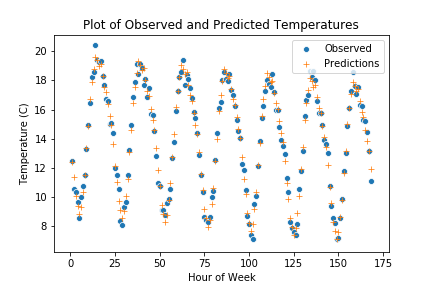
\includegraphics{figures/temps_on_train.png}
    \caption{Plot of predicted (x) and observed (o) temperatures on training data.}
    \label{fig:temperatures_on_train}
  \end{figure}
  \begin{figure}[!ht]
    \centering
    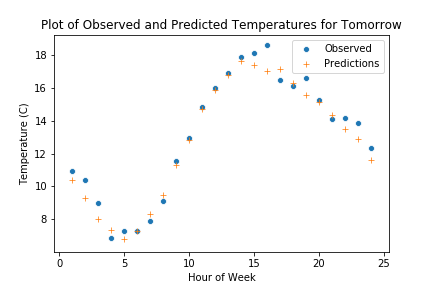
\includegraphics{figures/temps_on_test.png}
    \caption{Plot of predicted (x) and observed (o) temperatures on test data.}
    \label{fig:temperatures_on_test}
  \end{figure}

\newpage
\Q{Identifying a system from input/output data}

  \begin{solution}
    \begin{enumerate}[label=(\alph*)]
      \item We wish to find $A$ such that:
       \[
        J = \sum_{k=1}^N || Ax^{(k)} - y^{(k)}||^2
       \]
       is minimized. Taking the derivative wrt. $A$, we have:
       \begin{align*}
        \frac{\partial J}{\partial A} &= \frac{\partial}{\partial A} \left[\sum_{k=1}^N || Ax^{(k)} - y^{(k)}||^2 \right ] \\
        &= \sum_{k=1}^N \frac{\partial}{\partial A}\left[ || Ax^{(k)} - y^{(k)}||^2 \right ] \\
        &= \sum_{k=1}^N \frac{\partial}{\partial A}\left[ (Ax^{(k)} - y^{(k)})^T(Ax^{(k)} - y^{(k)}) \right ] \\
        &= 2\sum_{k=1}^N  (Ax^{(k)} - y^{(k)}) x^{(k)T} \\
        &= 2A \sum_{k=1}^N x^{(k)}x^{(k)T} - 2\sum_{k=1}^N  y^{(k)}x^{(k)T}
       \end{align*}
       So setting equal to $0$ and solving for $A$, we have:
       \begin{align*}
        A &= \left(\sum_{k=1}^N  y^{(k)}x^{(k)T}\right)\left(\sum_{k=1}^N x^{(k)}x^{(k)T} \right)^{-1}
       \end{align*}
       So we can find $A$ if and only if the second term above is invertible.

       \item Implementing the method discussed above, we obtain the following $A$:
       \[
        \hat{A} =
          \begin{bmatrix}
            2.02992454 &  5.02077879 &  5.01040266 \\
            0.0114300076 &  6.99991043 &  1.01061265 \\
            7.04239020 & 0 &  6.94476335 \\
            6.99765743 &  3.97592792 &  4.00242122 \\
            9.01295285 &  1.04493868 &  6.99800225 \\
            4.01187599 &  3.96488792 &  9.02674982 \\
            4.98710794 &  6.97233996 &  8.03363399 \\
            7.94249406 &  6.08754514 &  3.01735388 \\
            0 &  8.97218370 & -0.0385465462 \\
            1.06123427 &  8.02076138 &  7.02847693
          \end{bmatrix}
       \]
       This gives us a realtive error of $0.05814323689487761$.
    \end{enumerate}
  \end{solution}

\newpage
\Q{Robust regression using the Huber penalty function}

  \begin{solution}
    \begin{enumerate}[label=(\alph*)]
      \item This is a straight-forward application of weighed iterative least squares. In particular, our weight function is given by the below at iteration $k + 1$:

      \[
        w_i(a^{(k)},b^{(k)}) = \frac{H_{\delta}(a^{(k)}t_i + b^{(k)} - x_i)}{(a^{(k)}t_i + b^{(k)} - x_i)^2}
      \]
      We have to be a bit careful with the denominator to make sure it does not equal $0$. Once we have the weights defined, we can use the standard update equation given by:
      \[
          \begin{bmatrix}
            a^{(k+1)} \\
            b^{(k+1)}
          \end{bmatrix} = (A^TW(a^{(k)},b^{(k)})A)^{-1}A^TW(a^{(k)},b^{(k)})x
      \]
      where we have:
      \begin{align*}
        A &= \begin{bmatrix}
          t_1 & 1 \\
          \vdots & \vdots \\
          t_N & 1
        \end{bmatrix} \in \mathbb{R}^{N \times 2} \\
        W &= \begin{bmatrix}
          w_1(a, b) & 0 & \cdots & 0 \\
          0 & w_2(a,b) & \cdots & 0 \\
          \vdots & \vdots & \ddots & \vdots \\
          0 & 0 & \cdots & w_N(a,b)
        \end{bmatrix} \in \mathbb{R}^{N \times N}
      \end{align*}
    \item Applying the method above to ``huber\_penalty\_function\_data.m'', we arrive at the following parameter values with the Huber loss:
    \[
      a = -4.9920376, b = 23.5669247
    \]
    for a total Huber loss of $0.40706964531961987$.
    

    As for ordinary least squares, we have the following parameters:
    \[
      a = -3.94855818, b = 19.03697567
    \]
    A visualization of the results in presented in Figure \ref{fig:huber_fit}. We can see that the red line (Huber fit) matches the main data much more closely, since it is penalized less for the outliers. On the other hand, we see that the LS fit (green line) has to change slope and shift to try and accomodate the outlines, meaning the main datapints suffer.
    \end{enumerate}
  \end{solution}

  \begin{figure}
    \centering
    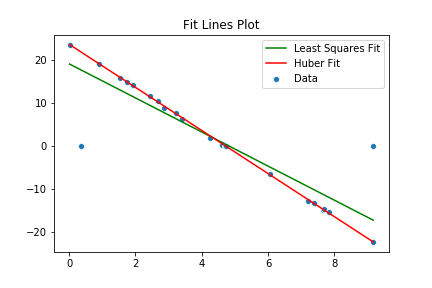
\includegraphics{line_plots_for_huber_fit.png}
    \caption{Plot of data as well as LS and Huber Fit}
    \label{fig:huber_fit}    
  \end{figure}

\newpage
\Q{Estimating a signal with interference}

  \begin{solution}
    \begin{enumerate}[label=(\alph*)]
      \item We now formalize each of the methods described:
        \begin{itemize}
          \item In Nikola's process, the estimate $\hat{x}_{\text{Nikola}}$ is given by:
            \[
              \hat{x}_{\text{Nikola}} = (A^TA)^{-1}A^Ty
            \]
            since it's just a straight-forward over-determined least squares problem. Note that this always has a solution if $A$ is full-rank.
          \item Almir's method consists of estimating both $\hat{x}_{\text{Almir}}$ and $\hat{v}$. Basically, this involves rewriting the problem $y = Ax + Bv$ as a single matrix, like below:
          \begin{align*}
            y &= Ax + Bv \\
            &= \begin{bmatrix} A & B \end{bmatrix}\begin{bmatrix} x \\ v \end{bmatrix} \\
            &= A'x'
          \end{align*}
          So now that we've presented it in this way, we have the solutions as:
          \[
            \begin{bmatrix}
              \hat{x}_{\text{Almir}} \\
              \hat{v}
            \end{bmatrix} = (A'^TA')^{-1}A'^Ty
          \]
          \item This method follows the same set-up as the method above, so we re-use $A' \in \mathbb{R}^{m \times (n + p)}$ and $x' \in \mathbb{R}^{(n+p)}$. Using the same process as described, we find $\hat{x}_{\text{Almir}}$ and $\hat{v}$.

          We then form the pseudo-measurement $\hat{y} = y - B\hat{v}$. We now have the system:
          \[
            \hat{y} = Ax
          \]
          and now find our \textit{true} estimate. Since this is just standard LS, we have:
          \[
            \hat{x}_{\text{Miki}} = (A^TA)^{-1}A^T\hat{y} = (A^TA)^{-1}A^T(y - B\hat{v})
          \]
        \end{itemize}
      \item First, we show that Miki and Nikola's methods are \textit{not} equivalent. In fact, let us consider the following system:
      \begin{align*}
        A &= \begin{bmatrix}
          1 \\
          0
        \end{bmatrix} \in \mathbb{R}^{2 \times 1} \\
        B &=
          \begin{bmatrix}
            1 \\
            1
          \end{bmatrix} \in \mathbb{R}^{2 \times 1}
      \end{align*}
      and let us suppose that we make the following measurement:
      \[
        y =
          \begin{bmatrix}
            2 \\
            1
          \end{bmatrix}
      \]
      By Nikola's method, we'll have the following $\hat{x}_{\text{Nikola}}$ estimate:
      \begin{align*}
        \hat{x}_{\text{Nikola}} &= (A^TA)^{-1}A^Ty \\
        &=
          \left(\begin{bmatrix}
            1 & 0
          \end{bmatrix}
          \begin{bmatrix}
            1 \\
            0
          \end{bmatrix}\right)^{-1}
          \begin{bmatrix}
            1 & 0
          \end{bmatrix}
          \begin{bmatrix}
            2 \\
            1
          \end{bmatrix} \\
          &= 2
      \end{align*}
      However, by Almir's method, we have:
      \begin{align*}
        \hat{x}_{\text{Almir}} &=
          \left(
            \begin{bmatrix}
              1 & 0 \\
              1 & 1
            \end{bmatrix}
            \begin{bmatrix}
              1 & 1 \\
              0 & 1
            \end{bmatrix}
          \right)^{-1}
            \begin{bmatrix}
              1 & 0 \\
              1 & 1
            \end{bmatrix}
            \begin{bmatrix}
              2 \\
              1
            \end{bmatrix} \\
          &= \left(
            \begin{bmatrix}
              1 & 1 \\
              1 & 2
            \end{bmatrix}
          \right)^{-1}
          \begin{bmatrix}
            2 \\
            3
          \end{bmatrix} \\
          &=
            \begin{bmatrix}
              2 & -1 \\
              -1 & 1
            \end{bmatrix}
            \begin{bmatrix}
            2 \\
            3
          \end{bmatrix} \\
        &= \begin{bmatrix}
            1 \\
            1
           \end{bmatrix}
      \end{align*}
      From the above, we can clearly see that $\hat{x}_{\text{Almir}} \neq \hat{x}_{\text{Nikola}}$. As such, these two methods are not equivalent.


      Next, we show that Miki's method is actually equivalent to Almir's method. That is, we show that $\hat{x}_{\text{Miki}} = \hat{x}_{\text{Almir}}$. First, we recall that $\hat{x}_{\text{Almir}}$ is is the unique solution satisfying the following system of equations:
      \begin{align*}
        A'^Ty &= A'^TA' \begin{bmatrix} \hat{x}_{\text{Almir}} \\ \hat{v} \end{bmatrix} \\
        \implies \begin{bmatrix} A & B \end{bmatrix}^Ty &= \begin{bmatrix} A & B \end{bmatrix}^T\begin{bmatrix} A & B \end{bmatrix} \begin{bmatrix} \hat{x}_{\text{Almir}} \\ \hat{v} \end{bmatrix} \tag{Definition of $A'$} \\
        \implies 
        \begin{bmatrix} 
          A^Ty \\
          B^Ty
        \end{bmatrix} &= 
        \begin{bmatrix}
        A^TA\hat{x}_{\text{Almir}} + A^TB\hat{v} \\
        B^TA\hat{x}_{\text{Almir}} + B^TB\hat{v}
        \end{bmatrix} \tag{Matrix Multiplication} \\
        \implies A^TB\hat{v} &= A^Ty - A^TA\hat{x}_{\text{Almir}} \tag{Taking just the top system}
      \end{align*}
      However, we note that following:
      \begin{align*}
        \hat{x}_{\text{Miki}} &= (A^TA)^{-1}A^T(y - B\hat{v}) \\
        &= (A^TA)^{-1}(A^Ty - A^TB\hat{v}) \tag{Distributing $A^T$} \\
        &= (A^TA)^{-1}(A^Ty - (A^Ty - A^TA\hat{x}_{\text{Almir}})) \tag{Subtituting results from above} \\
        &= (A^TA)^{-1 }(A^TA)\hat{x}_{\text{Almir}} \tag{Simplifying} \\ 
        &= \hat{x}_{\text{Almir}}
      \end{align*}
      As such, we can see that $\hat{x}_{\text{Miki}} = \hat{x}_{\text{Almir}}$ as expected.

      \item Almir's method works the best. It is equivalent to Miki's, but with less steps, and should provide better answers. Note that any solution $\hat{x}_{\text{Nikola}}$ will always lead to $\hat{y} \in \textbf{image}(A)$. However, with Almir's method, the only restriction is that $\hat{y} \in \textbf{image}(A) \bigcup \textbf{image}(B)$. As such, any observations $y$ where $B^Ty \neq 0$ will be better approximated by Almir's method (since it can accuraltey attribute some part of $y$ to the output space of $B$).

      However, it is interesting to note that Almir's method can be significantly more expensive than Nikola's, since it might require inverting a matrix that is twice as big.
    \end{enumerate}

  \end{solution}

\end{questions}

\includepdf[
    %% Include all pages of the PDF
    pages=-,
    %% make this page have the usual page style
    %% (you can change it to plain etc). By default pdfpages
    %% sets the pagecommand to \pagestyle{empty}
    pagecommand={\pagestyle{headings}}]
%% The pdf file itself
{HW4Code.pdf}















\end{document}
